\documentclass{article}
\usepackage[utf8]{inputenc}
\usepackage{tikz}
\usetikzlibrary{shapes.geometric, arrows}

\tikzstyle{startstop} = [rectangle, rounded corners, minimum width=3cm, minimum height=1cm,text centered, draw=black, fill=red!30]
\tikzstyle{io} = [trapezium, trapezium left angle=70, trapezium right angle=110, minimum width=3cm, minimum height=1cm, text centered, draw=black, fill=blue!30]
\tikzstyle{process} = [rectangle, minimum width=3cm, minimum height=1cm, text centered, text width=5 cm, draw=black, fill=orange!30]
\tikzstyle{decision} = [diamond, minimum width=3cm, minimum height=1cm, text centered, draw=black, fill=green!30]
\tikzstyle{arrow} = [thick,->,>=stealth]


\tikzstyle{node1} = [trapezium, trapezium left angle=45, trapezium right angle=45, rotate=90, minimum width=3cm, minimum height=1cm, text centered, draw=black, fill=purple!30]


\tikzstyle{node2} = [rectangle,minimum width=1.5cm, minimum height=5cm,text centered, draw=black, fill=green!30]

\tikzstyle{node3} = [rectangle,minimum width=1cm, minimum height=4cm,text centered, draw=black, fill=green!30]
\tikzstyle{node4} = [rectangle,minimum width=1cm, minimum height=5cm,text centered, draw=black, fill=purple!30]

\tikzstyle{node5} = [rectangle,minimum width=1cm, minimum height=10cm,text centered, draw=black, fill=red!30]

\tikzstyle{node6} = [circle,radius=2cm,text centered, draw=black, fill=white!30]


\begin{document}

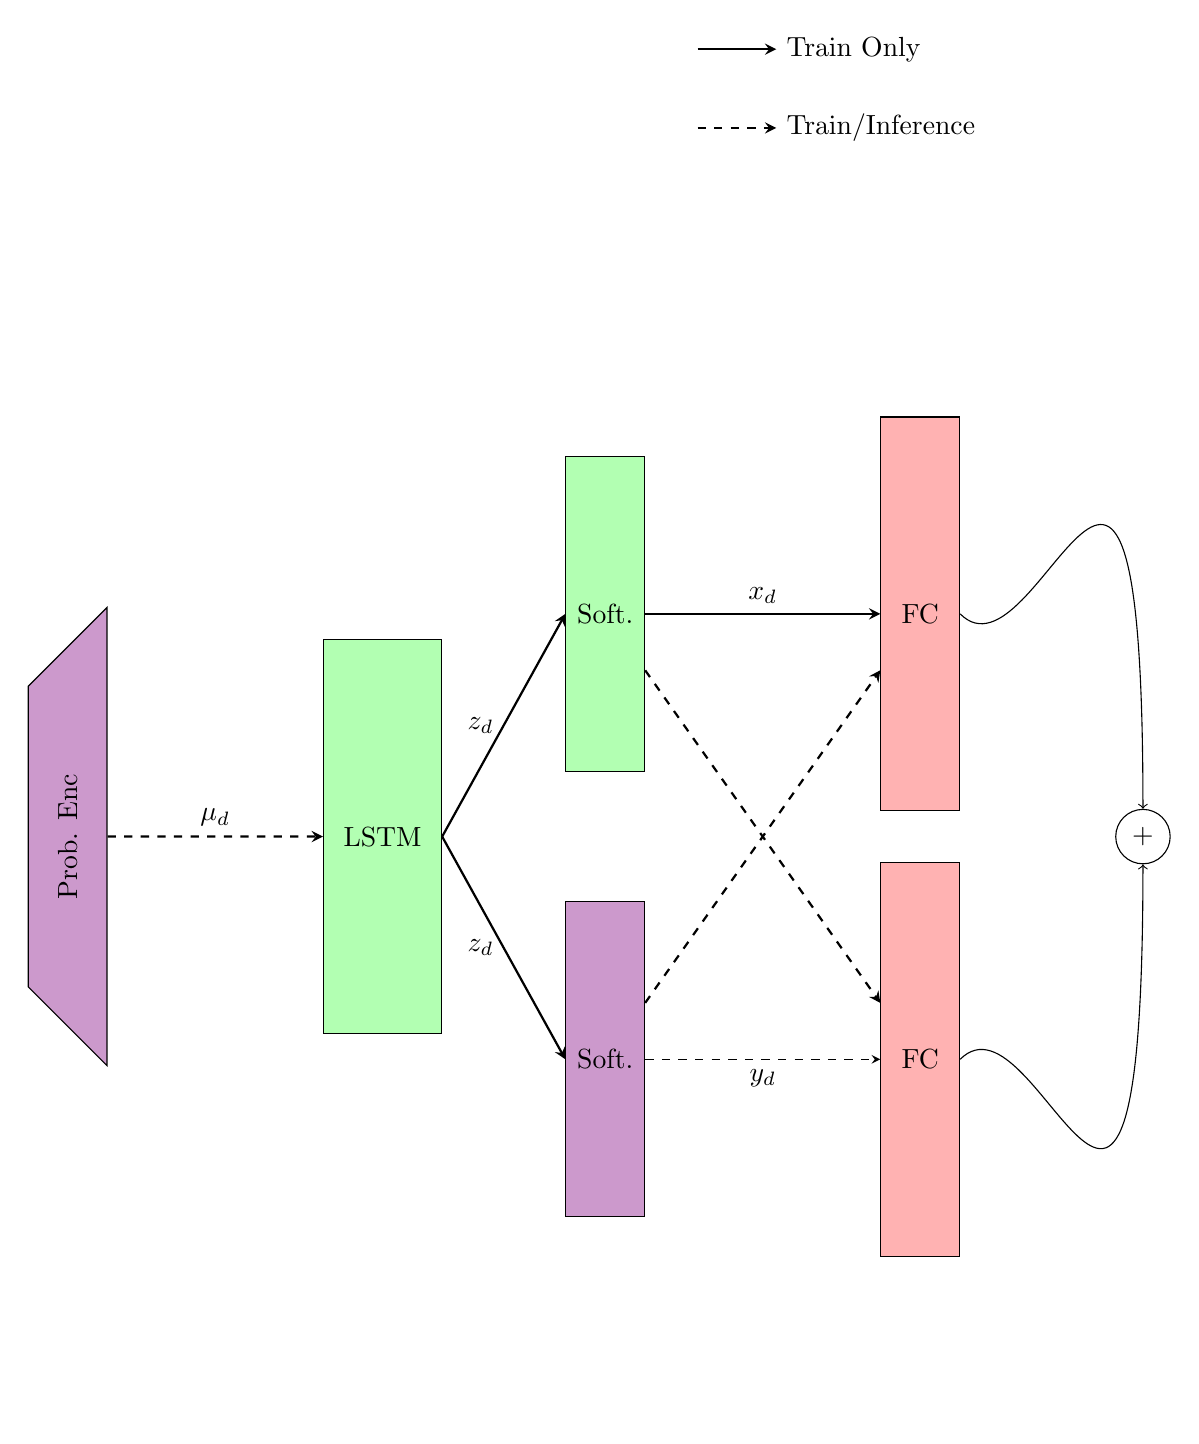
\begin{tikzpicture}[node distance=4cm]

\node (A) [node1, fill=violet!40] {Prob. Enc};
\node (B) [node2, right of=A]{LSTM}; 
\node (C) [node3, above right of=B]{Soft.}; 
\node (D) [node3, below right of=B,fill=violet!40]{Soft.};
\node (E) [node4, right of=C,fill=red!30]{FC};
\node (F) [node4,fill=red!30,  right of=D]{FC};
\node (F2) [node4,fill=red!30,  right of=D]{FC};
\node(G) [node6, below right of = E]{+};

\draw [->,thick,dashed,>=stealth ] (A) -- node[above] {$\mu_d$} (B);

\draw[->] (E.east) .. controls ++(1,-1) and ++(0, 7) .. (G.north);

\draw[->] (F.east) .. controls ++(1,1)  and ++(0, -7) .. (G.south);
\draw [->, dashed, thick, >=stealth] (C) --  (F);


\draw[->, thick, >=stealth] (B.east) -- node[left]{$z_d$} (C.west);
\draw[->, thick, >=stealth] (B.east) -- node[left]{$z_d$} (D.west);


\draw[->, thick, >=stealth] (C) -- node[above]{$x_d$} (E);
\draw[->, dashed, >=stealth] (D) -- node[below]{$y_d$} (F);

\draw [->, dashed, thick, >=stealth] (D) -- node[above] {}  (E);

\draw [->, thick, >=stealth](8,10) --(9,10) node[right]{Train Only};
\draw [->,dashed, thick, >=stealth](8,9) --(9,9) node[right]{Train/Inference};

\end{tikzpicture}


\end{document}



